\documentclass[12pt,fleqn]{article}\usepackage{../../common}
\begin{document}
Da�lar Aras�nda En Optimal Y�r�y�� Yolu Bulmak

\begin{minted}[fontsize=\footnotesize]{python}
from mpl_toolkits.mplot3d import Axes3D
from scipy.spatial.distance import cdist
from matplotlib import cm

def gfunc(x, y):
    s1 = 2.2; x1 = 2.0; y1 = 2.0
    g1 = np.exp( -4 *np.log(2) * ((x-x1)**2+(y-y1)**2) / s1**2)
    return g1 

D = 50

x = np.linspace(0,5,D)
y = np.linspace(0,5,D)

xx,yy = np.meshgrid(x,y)
print (xx.shape)
print (yy.shape)
zz = gfunc(xx,yy)

fig = plt.figure()
ax = fig.gca(projection='3d')
ax.set_xlim(0,5)
ax.set_ylim(0,5)
surf = ax.plot_wireframe(xx, yy, zz,rstride=10, cstride=10)

t = np.linspace(0,1.0,100)

a1,a2,a3 = 1.5, 10.1, 4.0
b1,b2,b3 = 0.3, 0.4, 30.3

a0,b0=(1.0,1.0)
ex,ey=(0.3,4.0)

a4 = ex - a0 - (a1+a2+a3)
b4 = ey - b0 - (b1+b2+b3)

x = a0 + a1*t + a2*t**2 + a3*t**3 + a4*t**4 
y = b0 + b1*t + b2*t**2 + b3*t**3 + b4*t**4

ax.plot3D(x, y, gfunc(x,y),'r.')

plt.savefig('calc_multi_40_elev_01.png')
\end{minted}

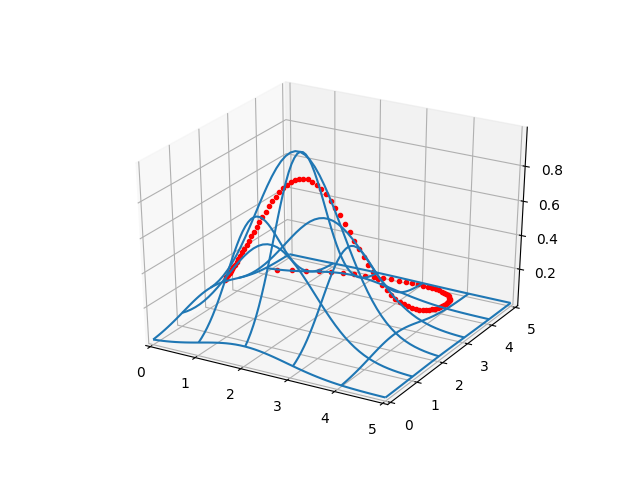
\includegraphics[width=20em]{calc_multi_40_elev_01.png}


\begin{minted}[fontsize=\footnotesize]{python}
print (gfunc(np.array([30,10,400]),np.array([10,20,200])))
\end{minted}

\begin{verbatim}
[1.07205709e-211 2.96055607e-097 0.00000000e+000]
\end{verbatim}


$$
\int_{t=0}^{t=1} f(x(t),y(t)) \sqrt{(\ud x/\ud t)^2 + (\ud y/\ud t)^2} \ud t
$$


\begin{minted}[fontsize=\footnotesize]{python}
def intval(t,a0,a1,a2,a3,a4,b0,b1,b2,b3,b4):
   sq = np.sqrt(b1 + 2*b2*t + 3*b3*t**2 - 112.0*t**3 + (a1 + 2*a2*t + 3*a3*t**2 - 65.2*t**3)**2)
   x = a0 + a1*t + a2*t**2 + a3*t**3 + a4*t**4 
   y = b0 + b1*t + b2*t**2 + b3*t**3 + b4*t**4
   x = np.array(x)
   y = np.array(y)   
   z = gfunc(x,y)   
   res = z * sq
   T = np.trapz(res, x=t)
   return T

t = np.linspace(0,1,100)
a0,a1,a2,a3 = 1.0, 1.5, 10.1, 4.0
b0,b1,b2,b3 = 1.0, 0.3, 0.4, 30.3

sx,sy=(a0,b0)
ex,ey=(0.3,4.0)

a4 = ex - sx - (a1+a2+a3)
b4 = ey - sy - (b1+b2+b3)

T = intval(t,a0,a1,a2,a3,a4,b0,b1,b2,b3,b4)
print (T)
\end{minted}

\begin{verbatim}
1.7109299071584967
\end{verbatim}






















\begin{minted}[fontsize=\footnotesize]{python}
import sympy

vars = 't a0 a1 a2 a3 b0 b1 b2 b3 gamma x y'
t, a0, a1, a2, a3, b0, b1, b2, b3, gamma, x, y = sympy.symbols(vars)

xdef = a0 + a1*t + a2*t**2 + a3*t**3 + a4*t**4
ydef = b0 + b1*t + b2*t**2 + b3*t**3 + b4*t**4

dxdt = sympy.diff(xdef,t)
print (dxdt)
dydt = sympy.diff(ydef,t)
print (dydt)
sqrtdef = sympy.sqrt(sympy.diff(xdef,t)**2 + sympy.diff(ydef,t))
print (sqrtdef)
\end{minted}

\begin{verbatim}
a1 + 2*a2*t + 3*a3*t**2 - 65.2*t**3
b1 + 2*b2*t + 3*b3*t**2 - 112.0*t**3
sqrt(b1 + 2*b2*t + 3*b3*t**2 - 112.0*t**3 + (a1 + 2*a2*t + 3*a3*t**2 - 65.2*t**3)**2)
\end{verbatim}


[devam edecek]

\end{document}
